\documentclass[tikz,border=5mm]{standalone}
\usepackage{xcolor}

\definecolor{trafficgreen}{RGB}{34, 139, 34}
\definecolor{trafficyellow}{RGB}{204, 170, 0}
\definecolor{gameblue}{RGB}{0, 102, 204}

\begin{document}
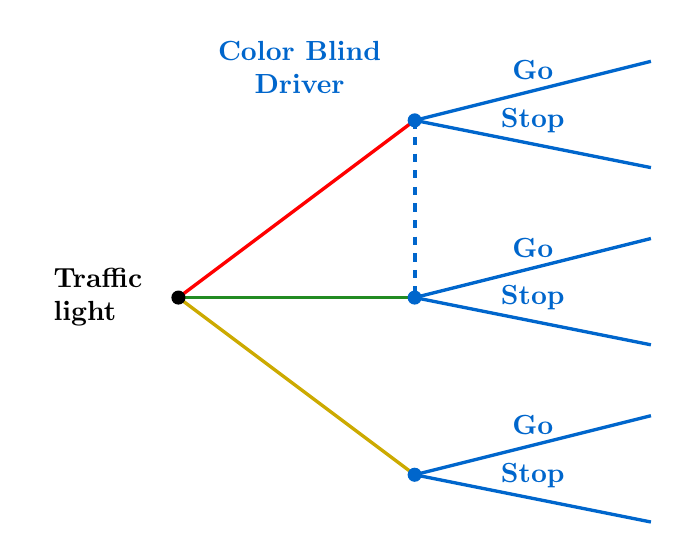
\begin{tikzpicture}[
    scale=1.5,
    font=\bfseries,
    dot/.style={circle, fill=#1, inner sep=1.8pt},
    dot/.default=black,
    line width=1.2pt
]

    % Coordinates
    \coordinate (root)       at (0, 0);
    \coordinate (driver_top) at (2, 1.5);
    \coordinate (driver_mid) at (2, 0);
    \coordinate (driver_bot) at (2, -1.5);
    
    \coordinate (l1_go)   at (4, 2.0);
    \coordinate (l1_stop) at (4, 1.1);
    
    \coordinate (l2_go)   at (4, 0.5);
    \coordinate (l2_stop) at (4, -0.4);
    
    \coordinate (l3_go)   at (4, -1.0);
    \coordinate (l3_stop) at (4, -1.9);

    % Level 1 branches (Traffic light signals)
    \draw[red] (root) -- (driver_top);
    \draw[trafficgreen] (root) -- (driver_mid);
    \draw[trafficyellow] (root) -- (driver_bot);

    % Information Set (Dashed Blue Line for Color Blind Driver)
    \draw[gameblue, dashed, line width=1.5pt] (driver_top) -- (driver_mid);

    % Level 2 branches (Color Blind Driver - Blue)
    \draw[gameblue] (driver_top) -- (l1_go)   node[midway, above] {Go};
    \draw[gameblue] (driver_top) -- (l1_stop) node[midway, above] {Stop};
    
    \draw[gameblue] (driver_mid) -- (l2_go)   node[midway, above] {Go};
    \draw[gameblue] (driver_mid) -- (l2_stop) node[midway, above] {Stop};
    
    \draw[gameblue] (driver_bot) -- (l3_go)   node[midway, above] {Go};
    \draw[gameblue] (driver_bot) -- (l3_stop) node[midway, above] {Stop};

    % Nodes & Labels
    \node[dot=black, align=left, label=left:\begin{tabular}{l}Traffic\\light\end{tabular}] at (root) {};
    \node[dot=gameblue, label={[gameblue]above left:\begin{tabular}{c}Color Blind\\Driver\end{tabular}}] at (driver_top) {};
    \node[dot=gameblue] at (driver_mid) {};
    \node[dot=gameblue] at (driver_bot) {};

\end{tikzpicture}
\end{document}
